\documentclass{paper}

%\usepackage{times}
\usepackage{epsfig}
\usepackage{graphicx}
\usepackage{amsmath}
\usepackage{amssymb}
\usepackage{color}
\usepackage{caption}
\usepackage{subcaption}


% load package with ``framed'' and ``numbered'' option.
%\usepackage[framed,numbered,autolinebreaks,useliterate]{mcode}

% something NOT relevant to the usage of the package.
\setlength{\parindent}{0pt}
\setlength{\parskip}{18pt}
\graphicspath{{images/}}


\usepackage[latin1]{inputenc}
\usepackage[T1]{fontenc}


\usepackage{listings}
\lstset{%
   language=Matlab,
   basicstyle=\small\ttfamily,
}



\title{Assignment 4}



\author{Jenni Simon\\09-116-005}
% //////////////////////////////////////////////////


\begin{document}



\maketitle


% Add figures:
%\begin{figure}[t]
%%\begin{center}
%\quad\quad   \includegraphics[width=1\linewidth]{ass2}
%%\end{center}
%
%\label{fig:performance}
%\end{figure}



\paragraph{Exercise 1}

Figure \ref{fig:male} and table \ref{tab:male} show the linear regression model
for the male examples and figure \ref{fig:female} and table \ref{tab:female} the
results for females. We observe that the estimated intercept  is significantly higher
for the female set, while the proportionality (linear coefficient in the model)
is only slightly greater compared to the male set.

The model therefore predicts women to have a higher wage compared to men given
the same amount of education.

\begin{figure}[!h]
  \begin{center}
    \quad\quad
    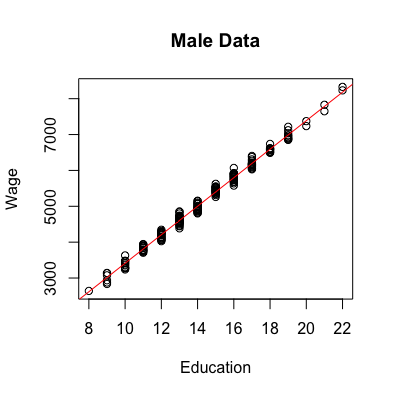
\includegraphics[width=.6\linewidth]{male_plot}
  \end{center}
  \caption{Plot showing years of education vs. wage for men. Linear regression
   model given by the red line.}
   \label{fig:male}
\end{figure}

\begin{table}[!h]
  \centering
    \caption{Linear regression model for men.}
    \label{tab:male}
    \begin{tabular}{|c|c|c|c|c|}
      \hline
                & Estimate  & Std. Error  & t-value & Pr(>|t|)    \\ \hline
      Intercept & -563.61    & 37.50      & -15.03  & <2e-16       \\ \hline
      Education & 397.54    & 2.58        & 154.10  & <2e-16      \\ \hline
    \end{tabular}
\end{table}

\begin{figure}[!h]
  \begin{center}
    \quad\quad
    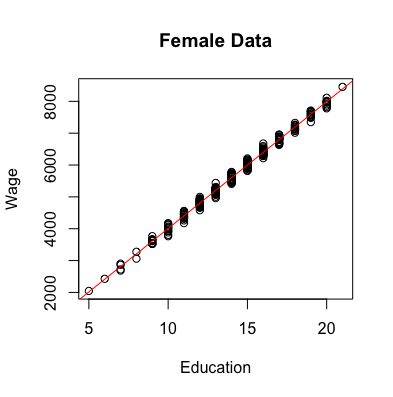
\includegraphics[width=.6\linewidth]{female_plot}
  \end{center}
  \caption{Plot showing years of education vs. wage for women. Linear regression
   model given by the red line.}
   \label{fig:female}
\end{figure}

\begin{table}[!h]
  \centering
    \caption{Linear regression model for women.}
    \label{tab:female}
    \begin{tabular}{|c|c|c|c|c|}
      \hline
                & Estimate  & Std. Error  & t-value  & Pr(>|t|)    \\ \hline
      Intercept & 24.199    & 27.937      &  0.866   & 0.387       \\ \hline
      Education & 398.250   & 1.919       &  207.559  & <2e-16      \\ \hline
    \end{tabular}
\end{table}



\paragraph{Exercise 2}
Looking at the description of the data, the following attributes can not be used to predict the performance:
\begin{itemize}
\item Vendor and model: As they are non-descriptive and non-exhaustive (not all vendors/models). Therefore useless for prediction.
\item PRP: The goal field.
\item ERP: The linear regression guesses.
\end{itemize}

\paragraph{Exercise 3}

Fitting a model using all possible predictors (excluding the ones from Ex2)
we choose the most significant variable, i.e. the one with the highest value
for $|t|$ or the lowest value for $P(>|t|)$ respectively. This turned out to be
the variable \textbf{MMAX}.

Table \ref{tab:confRPR} shows the confidence intervals for the estimated model
parameters. We are confident in observing a linear increase of PRP with MMAX.

\begin{table}[!h]
  \centering
    \caption{Confidence interval for the linear regression model $PRP\sim MMAX$.}
    \label{tab:confRPR}
    \begin{tabular}{|c|c|c|}
      \hline
                      & 2.5\%         & 97.5\%          \\ \hline
      Intercept       & -49.77265640  & -18.22582429    \\ \hline
      MMAX            & 0.01088673    & 0.01278561      \\ \hline
    \end{tabular}
\end{table}


\paragraph{Exercise 4}

Figure \ref{fig:prp_mmax} shows the found linear relationship.

\begin{figure}[!h]
  \begin{center}
    \quad\quad
    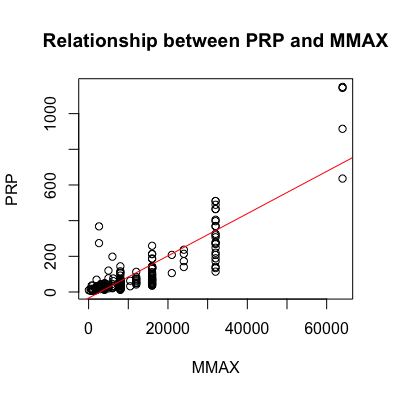
\includegraphics[width=.6\linewidth]{prp_mmax}
  \end{center}
  \caption{Plot showing MMAX vs. PRP. Linear regression
   model given by the red line.}
   \label{fig:prp_mmax}
\end{figure}


\paragraph{Exercise 5}
The data contained examples with NA values for the variable horsepower. These
examples have been removed from the dataset prior to further analysis.

The name of the car cannot be used because if we would use it, our model would
not be able to predict mpg for any previously unseen car-model. It is still
interesting to observe what happens when we incorporate the variable "name" in a
fit however: We observe that in cases where the name contains (diesel), the name
is actually very significant. This suggests that a categorical variable indicating
the fuel-type would be useful for the model.

It is a bit unclear how origin is defined, but it seems like it indicates whether the car was
produced in the USA (1), Asia (3) or Europe (2). As long as we do not want to predict mpg for cars
originating from outside of these zones (whatever that might be) and therefore assume
that all cars can be classified as having origin 1, 2 or 3, it makes sense to use this attribute.
Given the uncertainty of the definition however, it would be sensible to exclude this
variable.


\paragraph{Exercise 5}

Fitting a model using all possible predictors (excluding the ones from Ex4)
we choose the most significant variable. This turned out to be the variable \textbf{weight}.

Table \ref{tab:confMPG} shows the confidence intervals for the estimated model
parameters. We are confident in observing a linear decrease of mpg with weight.

\begin{table}[!h]
  \centering
    \caption{Confidence interval for the linear regression model $mpg\sim weight$.}
    \label{tab:confMPG}
    \begin{tabular}{|c|c|c|}
      \hline
                      & 2.5\%         & 97.5\%          \\ \hline
      Intercept       & 44.646282308  & 47.78676679    \\ \hline
      weight            & -0.008154515    & -0.00714017      \\ \hline
    \end{tabular}
\end{table}


\paragraph{Exercise 6}

Finally, figure \ref{fig:mpg} shows the found linear relationship.

\begin{figure}[!h]
  \begin{center}
    \quad\quad
    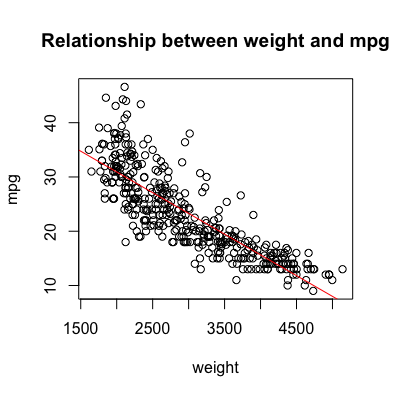
\includegraphics[width=.6\linewidth]{mpg}
  \end{center}
  \caption{Plot showing mpg vs. weight. Linear regression
   model given by the red line.}
   \label{fig:mpg}
\end{figure}

\end{document}
